\chapter{Linear Normal Form}
\label{chap:linear-normal-form}

A linear normal form separates two questions about a periodic accelerator:
what shape does an oscillation have in physical phase space, and by how much
does its phase advance each turn? A canonical change of coordinates answers
the first question; a rotation in those coordinates answers the second.
The familiar Courant--Snyder construction is the one-degree-of-freedom
version of this separation. An eigenvalue problem gives the same construction
for coupled motion in several degrees of freedom.

We first derive the normal form with matrices. We then write precisely the
same construction with compositional maps and Lie operators, using the
conventions of the preceding chapter. This establishes the starting point
for the nonlinear normal form: replace the linear change of coordinates by
a nonlinear canonical map, and replace constant rotations by more general
normal-form dynamics. The map-based approach is developed systematically
in Refs.~\cite{Forest_book1,Forest_book2}.



\section{The closed orbit is the origin of the normal form}
\label{sec:lnf-closed-orbit}

Choose an observation point $z$ in the ring and let $\mathcal M$ denote its
one-turn point map. Use paired canonical coordinates
\begin{equation}
    \vec z = (q_1,p_1,\ldots,q_d,p_d)^T,
    \qquad \vec z_{n + 1} = \mathcal M(\vec z_n)\,,
\end{equation}
where $n$ is the turn number. Usually $d = 2$ for transverse motion at fixed
momentum, or $d = 3$ when synchrotron motion is included. The closed orbit
$\vec z_{\rm co}$ is a fixed point:
\begin{equation}\label{eq:lnf-fixed-point}
    \mathcal M(\vec z_{\rm co}) = \vec z_{\rm co}\,.
\end{equation}
It need not coincide with the zero coordinates of the tracking model.
Alignment errors, corrector settings, dispersion, and nonlinear feed-down
can all make that distinction essential.

Define the deviation and the linear one-turn matrix (see
Eq.~\eqref{eq:pushforward}) by
\begin{equation}\label{eq:lnf-deviation}
    \vec\xi = \vec z-\vec z_{\rm co},
    \qquad M = \left.D\mathcal M\right|_{\vec z_{\rm co}}\,.
\end{equation}
Taylor expansion about the fixed point gives
\begin{equation}\label{eq:lnf-linearisation}
    \mathcal M(\vec z_{\rm co} + \vec\xi) = \vec z_{\rm co} + M\vec\xi + \mathcal O(\|\vec\xi\|^2),
    \qquad
    \vec\xi_{n + 1} = M\vec\xi_n + \mathcal O(\|\vec\xi_n\|^2)\,.
\end{equation}
Thus the linear normal form acts on the tangent motion around the closed
orbit, rather than on the absolute tracking coordinates. Even a lattice
containing nonlinear magnets has such a linearisation; its matrix includes
their derivatives evaluated on that orbit.

For an exactly affine map $\mathcal M(\vec z) = \vec d + M\vec z$, the orbit
satisfies
\begin{equation}
    (I-M)\vec z_{\rm co} = \vec d\,.
\end{equation}
For a nonlinear map, the corresponding Newton step is
\begin{equation}\label{eq:lnf-newton}
    \vec z^{(r + 1)} = \vec z^{(r)} + (I-D\mathcal M|_{\vec z^{(r)}})^{-1}
    \bigl[\mathcal M(\vec z^{(r)})-\vec z^{(r)}\bigr]\,.
\end{equation}
In code the inverse denotes a linear solve. A unit eigenvalue makes this
solve singular and requires a suitable constraint or a reduced problem.
For example, without RF there may be no isolated longitudinal fixed point;
one normally solves a transverse closed orbit for a prescribed momentum
offset instead of applying a three-mode rotation construction blindly.

\emph{Subtract the closed orbit before applying the normalisation.}
If $A$ is the matrix constructed below, the normalised coordinates are
$\vec w = A^{-1}(\vec z-\vec z_{\rm co})$. Using $A^{-1}\vec z$ instead
introduces a constant offset, so the apparent actions oscillate even when
the linear dynamics is perfectly stable. Computing the Jacobian at the
wrong origin can also give incorrect tunes and optics.



\section{Symplectic matrices and the eigenvalue problem}
\label{sec:lnf-eigenproblem}

With the canonical ordering above, we know from
Eq.~\eqref{eq:symplectic-jacobian} that:
\begin{equation}\label{eq:lnf-symplectic-matrix}
    M^T S M = S\,.
\end{equation}
This follows by differentiating the symplectic one-turn map
at its fixed point. It assumes Hamiltonian tracking without damping or
other non-symplectic processes. It also assumes genuinely canonical
coordinates. A longitudinal tracking variable called $\delta$ is not
automatically the momentum conjugate to the variable called $\zeta$;
the sign and any required change of variable must be established before
using this $S$ in six dimensions.

The normal-mode problem is
\begin{equation}\label{eq:lnf-eigenvalue}
    M\vec v_j = \lambda_j\vec v_j\,.
\end{equation}
Because $M$ is real and symplectic, eigenvalues occur with their complex
conjugates and reciprocals. For stable elliptic motion they lie on the
unit circle and can be written
\begin{equation}
    \lambda_j = \e^{\ii\mu_j},\qquad
    \overline{\lambda_j} = \e^{-\ii\mu_j}\,.
\end{equation}
The rotation normal form used here requires a complete eigenbasis:
the eigenvalues must be semisimple, meaning that their Jordan blocks have
size one. Unit-modulus eigenvalues alone are insufficient, since a
nontrivial Jordan block produces secular growth. In the derivation below
we take the modes to be distinct and away from $\lambda = \pm1$.
Semisimple degeneracies can also be treated, but require choosing a
symplectic basis within the degenerate eigenspace. Hyperbolic modes and
non-semisimple cases have other normal forms and do not conserve the
positive oscillator actions introduced here.

An ordinary eigensolver leaves the eigenvectors with an arbitrary complex
scale. Euclidean normalisation is not the normalisation needed for
canonical coordinates. Write
\begin{equation}
    \vec v_j = \vec u_j + \ii\vec t_j,
    \qquad
    \sigma_j = \frac{\vec v_j^\dagger S\vec v_j}{2\ii} = \vec u_j^T S\vec t_j\,.
\end{equation}
For a simple elliptic eigenvalue away from $\lambda = \pm 1$, $\sigma_j$ is
real and, under the non-degeneracy assumptions used here, nonzero.  Its sign is the convention-dependent symplectic (Krein) signature of the
chosen member of the conjugate pair. Select the
member of each conjugate pair for which $\sigma_j>0$; if needed replace
$(\lambda_j,\vec v_j)$ by
$(\overline{\lambda_j},\overline{\vec v_j})$. Then rescale
$\vec v_j\mapsto\vec v_j/\sqrt{\sigma_j}$, giving
\begin{equation}\label{eq:lnf-eigenvector-normalisation}
    \vec v_j^\dagger S\vec v_j = 2\ii,
    \qquad \vec u_j^T S\vec t_j = 1\,.
\end{equation}
This selection fixes the orientation of each canonical mode, so the
phase advance $\mu_j$ must be taken from the selected eigenvalue.
It need not be the positive principal angle returned by a library.

The symplectic orthogonality of different modes follows directly from
the eigenproblem. If $M\vec v = \lambda\vec v$ and
$M\vec r = \rho\vec r$, then
\begin{equation}
    \vec v^T S\vec r = \vec v^T M^T S M\vec r = \lambda\rho\,\vec v^T S\vec r\,.
\end{equation}
Consequently $\vec v^T S\vec r = 0$ when $\lambda\rho\ne1$.
Together with Eq.~\eqref{eq:lnf-eigenvector-normalisation}, these relations
make the real matrix
\begin{equation}\label{eq:lnf-normalisation-matrix}
    A = (\vec u_1,\vec t_1,\ldots,\vec u_d,\vec t_d)
    \qquad\text{satisfy}\qquad A^T S A = S\,.
\end{equation}
In exact arithmetic no further correction is needed for distinct modes;
numerical implementations should check the residual.

Taking real and imaginary parts of the eigenvalue equation gives
\begin{align}
    M\vec u_j& = \cos\mu_j\,\vec u_j-\sin\mu_j\,\vec t_j,\\
    M\vec t_j& = \sin\mu_j\,\vec u_j + \cos\mu_j\,\vec t_j\,.
\end{align}
Collecting these columns produces the desired decomposition:
\begin{equation}\label{eq:lnf-matrix-normal-form}
    M = A R A^{-1},\qquad
    R = \diag\bigl(R_2(\mu_1),\ldots,R_2(\mu_d)\bigr),
    \qquad
    R_2(\mu) = \begin{pmatrix}
    \cos\mu&\sin\mu\\-\sin\mu&\cos\mu
    \end{pmatrix}\,.
\end{equation}
The canonical inverse can also be written $A^{-1} = -S A^T S$.
This is a matrix derivation of the normal form, and also an explanation
of why it is an eigenvalue problem: eigenvalues provide the phase
advances, while normalised eigenvectors provide the phase-space basis.



\section{Normalisation and rotation do different jobs}
\label{sec:lnf-geometry-dynamics}

Define normalised Cartesian coordinates by
\begin{equation}\label{eq:lnf-normalised-coordinates}
    \vec w = (Q_1,P_1,\ldots,Q_d,P_d)^T = A^{-1}\vec\xi\,.
\end{equation}
Their linear dynamics is simply $\vec w_{n + 1} = R\vec w_n$.
Each mode therefore has an invariant action
\begin{equation}\label{eq:lnf-action}
    J_j = \frac{Q_j^2 + P_j^2}{2}\,.
\end{equation}
With our orientation of the rotation, write
\begin{equation}\label{eq:lnf-action-angle}
    Q_j = \sqrt{2J_j}\cos\phi_j,
    \qquad P_j = -\sqrt{2J_j}\sin\phi_j\,.
\end{equation}
Then $\poisson{\phi_j}{J_k} = \delta_{jk}$ and
\begin{equation}
    J_{j,n + 1} = J_{j,n},\qquad
    \phi_{j,n + 1} = \phi_{j,n} + \mu_j\pmod{2\pi}\,.
\end{equation}
The phase is undefined at $J_j = 0$, although the Cartesian normal form
remains regular there.

The matrix $A$ describes the geometry of the oscillations. It maps
normalised circles into physical ellipses and embeds the independent
modes in physical coordinates. Its inverse gives the normalised,
decoupled coordinates. The matrix $R$ describes the dynamics on those circles.
For several nonzero actions, the product of circles is a torus; $A$ embeds
that torus in physical phase space and $R$ translates its angles.
The complete linear solution is
\begin{equation}\label{eq:lnf-solution}
    \vec z_n = \vec z_{\rm co} + A R^n A^{-1}
    (\vec z_0-\vec z_{\rm co})\,.
\end{equation}

\begin{figure}[htbp]
\centering
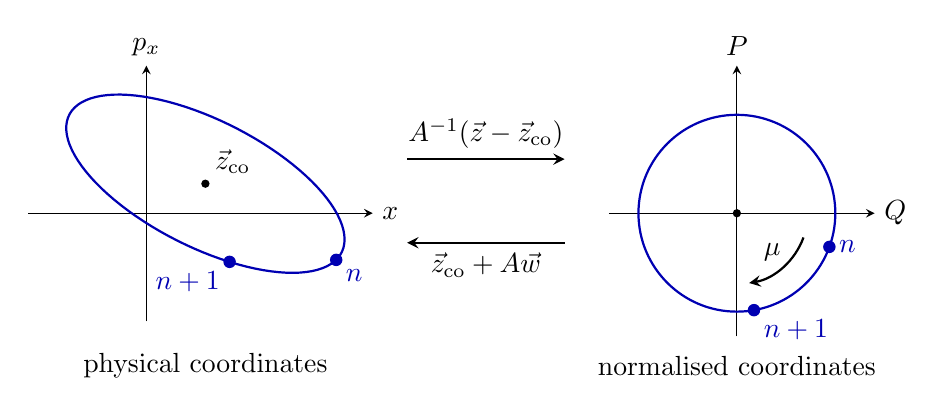
\begin{tikzpicture}[scale=1.25,>=stealth]
 \draw[->] (-1.2,0) -- (2.3,0) node[right] {$x$};
 \draw[->] (0,-1.1) -- (0,1.5) node[above] {$p_x$};
 \draw[blue!70!black,thick,domain=0:360,samples=100,variable=\t]
   plot ({0.6+1.414*cos(\t)},{0.3-0.566*cos(\t)-0.707*sin(\t)});
 \fill (0.6,0.3) circle (1.2pt);
 \node[above right] at (0.6,0.3) {$\vec z_{\rm co}$};
 \fill[blue!70!black] (1.929,-0.474) circle (1.8pt)
   node[below right] {$n$};
 \fill[blue!70!black] (0.846,-0.494) circle (1.8pt)
   node[below left] {$n + 1$};
 \node at (0.6,-1.55) {physical coordinates};
 \draw[->,thick] (2.65,0.55) -- (4.25,0.55)
   node[midway,above] {$A^{-1}(\vec z-\vec z_{\rm co})$};
 \draw[<-,thick] (2.65,-0.3) -- (4.25,-0.3)
   node[midway,below] {$\vec z_{\rm co} + A\vec w$};
 \begin{scope}[shift={(6,0)}]
   \draw[->] (-1.3,0) -- (1.4,0) node[right] {$Q$};
   \draw[->] (0,-1.25) -- (0,1.5) node[above] {$P$};
   \draw[blue!70!black,thick] (0,0) circle (1);
   \fill (0,0) circle (1.2pt);
   \fill[blue!70!black] ({cos(20)},{-sin(20)}) circle (1.8pt)
     node[right] {$n$};
   \fill[blue!70!black] ({cos(80)},{-sin(80)}) circle (1.8pt)
     node[below right] {$n + 1$};
   \draw[->,thick] ({0.72*cos(20)},{-0.72*sin(20)})
     arc[start angle=-20,end angle=-80,radius=0.72];
   \node at (0.36,-0.4) {$\mu$};
   \node at (0,-1.55) {normalised coordinates};
 \end{scope}
\end{tikzpicture}
\caption{The normalisation centres the orbit and changes its ellipse into
a circle. The rotation advances the phase on that circle. These are
separate parts of the one-turn map.}
\label{fig:lnf-geometry-dynamics}
\end{figure}

The normalisation is not unique. Multiplying an eigenvector by
$\e^{\ii\theta_j}$ rotates its two real columns, and replacing $A$ by
$A G$ with $G = \diag(R_2(\theta_1),\ldots,R_2(\theta_d))$ leaves
$A R A^{-1}$ unchanged. This is a choice of phase origin, often called
a phase gauge. Mode permutations also leave the physical matrix
unchanged. A useful convention fixes one nonzero coordinate component
of each eigenvector to be real and positive. In a parameter scan, modes
and phases should instead be continued smoothly from the previous point.
Such conventions affect individual normal-form coefficients, but not
the physical map, actions, or eigenvalues.



\section{Beta functions, phase advances, and tunes}
\label{sec:lnf-beta-tune}

\subsection{One uncoupled degree of freedom}

For an uncoupled pair $(x,p_x)$, choose the triangular Courant--Snyder
normalisation
\begin{equation}\label{eq:lnf-courant-snyder}
    A_{\rm CS} = \begin{pmatrix}
        \sqrt{\beta} & 0 \\
        -\frac{\alpha}{\sqrt{\beta}} & \frac{1}{\sqrt{\beta}}
    \end{pmatrix},\qquad
    \begin{pmatrix}
        Q\\P
    \end{pmatrix} = \begin{pmatrix}
        \frac{x-x_{\rm co}}{\sqrt{\beta}} \\
        \frac{\alpha(x-x_{\rm co}) + \beta(p_x-p_{x,\rm co})}{\sqrt{\beta}}
    \end{pmatrix}\,.
\end{equation}
Here $p_x$ is the canonical momentum used in the model; identifying it
with the geometric slope requires the corresponding paraxial convention.
Set $\gamma = (1 + \alpha^2)/\beta$. Direct multiplication of
$A_{\rm CS}R_2(\mu)A_{\rm CS}^{-1}$ gives
\begin{equation}\label{eq:lnf-twiss-matrix}
    M = \begin{pmatrix}
    \cos\mu + \alpha\sin\mu&\beta\sin\mu\\
    -\gamma\sin\mu&\cos\mu-\alpha\sin\mu
    \end{pmatrix}\,.
\end{equation}
Thus, away from $\sin\mu = 0$,
\begin{equation}
    \cos\mu = \tfrac12\Tr M,\qquad
    \beta = \frac{M_{12}}{\sin\mu},\qquad
    \alpha = \frac{M_{11}-M_{22}}{2\sin\mu}\,.
\end{equation}
The sign of $\sin\mu$ is chosen to give $\beta>0$.
The invariant in physical deviations is
\begin{equation}\label{eq:lnf-cs-invariant}
    2J = \gamma(x-x_{\rm co})^2 + 2\alpha(x-x_{\rm co})(p_x-p_{x,\rm co}) + \beta(p_x-p_{x,\rm co})^2\,.
\end{equation}
In particular $x-x_{\rm co} = \sqrt{2\beta J}\cos\phi$.
The beta function controls the oscillation amplitude at fixed action;
it is a property of the normalisation, whereas the tune is a property
of the rotation:
\begin{equation}\label{eq:lnf-tune}
    \nu_j = \frac{\mu_j}{2\pi}\,.
\end{equation}
A one-turn eigenvalue fixes $\nu_j$ only modulo an integer. Recovering
the accumulated tune requires following the phase through the ring or
continuing it from a known lattice. Applying $\arccos(\Tr M/2)$ alone
loses both the orientation and this phase branch.


\subsection{Coupled modes and transport around the ring}

In a coupled lattice, a physical coordinate contains contributions from
several normal modes. If row $r$ of $A$ corresponds to a position
coordinate $x_r$, define the projected mode beta functions
\begin{equation}\label{eq:lnf-mode-beta}
    \beta_{rj} = A_{r,2j-1}^2 + A_{r,2j}^2\,.
\end{equation}
Indeed,
\begin{align}
    x_r-x_{r,\rm co}
    & = \sum_{j = 1}^{d}\sqrt{2J_j}
    \bigl[A_{r,2j-1}\cos\phi_j-A_{r,2j}\sin\phi_j\bigr],\\
    \mean{(x_r-x_{r,\rm co})^2}_{\vec\phi}
    & = \sum_j\beta_{rj}J_j\,.
\end{align}
The average is over independent mode phases. A phase-mixed beam with
$\mean{J_j} = \epsilon_j$ therefore has
$\sigma_{x_r}^2 = \sum_j\beta_{rj}\epsilon_j$ in this linear model.
These projected functions are invariant under the phase gauge above.
They reduce to the usual beta function for an uncoupled mode, but a
coupled lattice generally needs several such functions rather than a
single horizontal and a single vertical beta.
For a detailed eigenmode treatment see Wolski's formulation of coupled
linear optics~\cite{WolskiCoupled2006}.

Let $L(s_2,s_1)$ be the Jacobian of the point map between two locations,
evaluated along their closed orbit. At each location choose a local
phase convention for $A(s)$. The transfer matrix has the form
\begin{equation}\label{eq:lnf-local-transport}
    L(s_2,s_1) = A(s_2)
    \diag\bigl(R_2(\Delta\psi_1),\ldots,R_2(\Delta\psi_d)\bigr)
    A(s_1)^{-1}\,.
\end{equation}
This expresses the same separation along the whole ring: local optics
resides in $A(s)$ and accumulated phase resides in $\Delta\psi_j$.
At one full turn, periodic $A(s)$ gives the phases $\mu_j$.
Transporting the eigenvectors without removing their accumulating phases
is also possible, but then that phase is contained in the columns of
$A$ rather than displayed separately in the rotations.



\section{Phasors and the resonance basis}
\label{sec:lnf-phasors}

Complex normalised coordinates diagonalize the rotation itself. Define
the phasor and its conjugate by
\begin{equation}\label{eq:lnf-phasor}
    a_j = \frac{Q_j-\ii P_j}{\sqrt2} = \sqrt{J_j}\,\e^{\ii\phi_j},\qquad
    \bar a_j = \frac{Q_j + \ii P_j}{\sqrt2},\qquad
    J_j = a_j\bar a_j\,.
\end{equation}
They satisfy
\begin{equation}
    \poisson{a_j}{\bar a_k} = \ii\delta_{jk},\qquad
    a_{j,n + 1} = \e^{\ii\mu_j}a_{j,n},\qquad
    \bar a_{j,n + 1} = \e^{-\ii\mu_j}\bar a_{j,n}\,.
\end{equation}
The complex variables are a computational basis; physical phase-space
points still obey $\bar a_j = \overline{a_j}$.

More generally, for nonnegative multi-indices
$\vec k,\vec l$, use monomials
\begin{equation}\label{eq:lnf-resonance-monomial}
    m_{\vec k\vec l} = \prod_j a_j^{k_j}\bar a_j^{l_j} = \prod_j J_j^{(k_j + l_j)/2}
    \e^{\ii(\vec k-\vec l)\cdot\vec\phi}\,.
\end{equation}
Under substitution of the rotation they are eigenfunctions:
\begin{equation}\label{eq:lnf-resonance-basis}
    m_{\vec k\vec l}\circ\mathcal R = \e^{\ii(\vec k-\vec l)\cdot\vec\mu}
    m_{\vec k\vec l},
    \qquad \mathcal R(\vec w) = R\vec w\,.
\end{equation}
This is the \emph{resonance basis}. Unlike real Cartesian monomials,
whose coefficients mix under a rotation, each of these monomials only
acquires one known phase factor.

Writing $\vec m = \vec k-\vec l$, a discrete-turn
resonance occurs when
\begin{equation}\label{eq:lnf-resonance}
    \vec m\cdot\vec\mu = 2\pi r,
    \qquad\text{or equivalently}\qquad
    \vec m\cdot\vec\nu = r,
    \quad r\in\mathbb Z\,.
\end{equation}
Action monomials have $\vec k = \vec l$ and are invariant
for every tune. Nonzero $\vec m$ instead describes an angle
harmonic. For example $a_x^4$ has harmonic $4\phi_x$ and becomes
invariant at $4\nu_x\in\mathbb Z$; $a_x\bar a_y$ carries
$\phi_x-\phi_y$ and is associated with a difference resonance.
A real Hamiltonian contains conjugate pairs of such coefficients.

The resonance condition alone does not make a stable linear oscillator
unstable. It identifies harmonics that a perturbation can drive.
In the next chapter, removing a nonresonant harmonic requires dividing
by a factor proportional to
$1-\e^{\ii\vec m\cdot\vec\mu}$.
This factor vanishes on a resonance and becomes small nearby, explaining
both the usefulness of the phasor basis and the need to retain resonant
terms in the normal form.



% \section{An implementation with matrices}
% \label{sec:lnf-pseudocode}

% The following pseudocode assumes distinct elliptic modes and canonical
% coordinates. The routine \texttt{Jacobian} may use derivatives propagated
% through tracking, automatic differentiation, Taylor maps, or sufficiently
% accurate finite differences. The map and its Jacobian must use the same
% observation point, parameters, and coordinate convention.

% \begin{lstlisting}[basicstyle=\ttfamily\small,breaklines=true,columns=fullflexible]
% function linear_normal_form(one_turn_map, initial_orbit, tolerances):
%     zco = initial_orbit
%     repeat until orbit_residual is small:
%         residual = one_turn_map(zco) - zco
%         M = Jacobian(one_turn_map, zco)
%         step = solve(I - M, residual)
%         zco = zco + step
%     assert norm(one_turn_map(zco) - zco) < tolerances.orbit

%     M = Jacobian(one_turn_map, zco)       # Re-evaluate at converged orbit
%     S = block_diagonal([[0, 1], [-1, 0]], number_of_modes)
%     assert norm(transpose(M)*S*M - S) < tolerances.symplectic

%     eigenvalues, eigenvectors = eig(M)
%     pairs = pair_complex_conjugates(eigenvalues, eigenvectors)
%     assert stable_semisimple_elliptic_modes(pairs)
%     A = empty_real_matrix()
%     mu = empty_list()
%     for lambda, v in choose_one_member_of_each_pair(pairs):
%         sigma = real(conjugate_transpose(v)*S*v / (2*i))
%         if sigma < 0:
%             lambda, v = conjugate(lambda), conjugate(v)
%             sigma = -sigma
%         assert sigma > tolerances.mode_norm
%         v = v / sqrt(sigma)
%         v = choose_phase_gauge(v)  # Preserve its symplectic norm
%         append_columns(A, real(v), imag(v))
%         append(mu, argument(lambda))

%     A, mu = label_modes_and_continue_phases(A, mu)
%     R = block_diagonal(rotation(mu[j]) for each mode j)
%     assert norm(transpose(A)*S*A - S) < tolerances.normalisation
%     assert norm(M*A - A*R) < tolerances.factorization
%     return zco, A, mu

% function analyze_particle(z, zco, A):
%     w = solve(A, z - zco)     # Closed-orbit subtraction first
%     for each canonical pair Q, P in w:
%         J = (Q*Q + P*P)/2
%         phi = atan2(-P, Q)    # Defined only for nonzero action
%         report(J, phi)

% function propagate_linear(z, zco, A, mu, turns):
%     w = solve(A, z - zco)
%     w = block_diagonal(rotation(turns*mu[j]) for each mode j)*w
%     return zco + A*w
% \end{lstlisting}

% The last two residual checks establish different facts: $A^TSA = S$
% checks that the new coordinates are canonical, and $BA = AR$ checks
% that they reduce the dynamics to rotations. A small eigenvalue
% residual alone establishes neither the chosen symplectic scale nor
% the correct mode orientation. For a nonlinear tracking map, the
% linear propagation agrees locally to first order, and the actions
% computed with $A$ need not remain exactly constant at finite amplitude.



\section{The same normal form written as maps}
\label{sec:lnf-maps}

\subsection{Conjugating point maps}

Introduce the translation, linear normalisation, and their composition:
\begin{equation}\label{eq:lnf-embedding}
    \mathcal T_{\rm co}(\vec\xi) = \vec z_{\rm co} + \vec\xi,
    \qquad \mathcal L_A(\vec w) = A\vec w,
    \qquad \mathcal C_0 = \mathcal T_{\rm co}\circ\mathcal L_A\,.
\end{equation}
For each fixed closed orbit the translation is canonical, and $\mathcal L_A$
is canonical because $A^TSA = S$. The normalised full point map is
\begin{align}\label{eq:lnf-normalised-map}
    \mathcal F
    & = \mathcal L_A^{-1}\circ\mathcal T_{\rm co}^{-1}
    \circ\mathcal M\circ\mathcal T_{\rm co}\circ\mathcal L_A,\\
    \mathcal F(\vec w)
    & = A^{-1}\bigl[\mathcal M(\vec z_{\rm co} + A\vec w)-\vec z_{\rm co}\bigr]\,.
\end{align}
The rightmost point map acts first. By construction
\begin{equation}
    \mathcal F(\vec0) = \vec0,\qquad D\mathcal F|_{\vec0} = R,
    \qquad \mathcal F(\vec w) = R\vec w + \mathcal O(\|\vec w\|^2)\,.
\end{equation}
For an affine symplectic $\mathcal M$, this is exactly $\mathcal R$ and
\begin{equation}\label{eq:lnf-map-factorization}
    \mathcal M = \mathcal C_0\circ\mathcal R\circ\mathcal C_0^{-1}\,.
\end{equation}
For a nonlinear map the same equation holds for its affine approximation
$\mathcal M_{\rm lin}(\vec z) = \vec z_{\rm co} + M(\vec z-\vec z_{\rm co})$.
Thus matrix similarity has become canonical conjugacy of point maps.
The argument $\vec z_{\rm co} + A\vec w$ makes explicit both the orbit
subtraction and the direction of the normalisation.

For substitution operators
$\widehat{\mathcal U}g = g\circ\mathcal U$, the composition order reverses
as in Eq.~\eqref{eq:pullback-order}. Consequently
\begin{equation}\label{eq:lnf-pullback-normal-form}
    \widehat{\mathcal F} = \widehat{\mathcal C_0}\,
    \widehat{\mathcal M}\,
    \widehat{\mathcal C_0^{-1}},\qquad
    \widehat{\mathcal M_{\rm lin}} = \widehat{\mathcal C_0^{-1}}\,
    \widehat{\mathcal R}\,
    \widehat{\mathcal C_0}\,.
\end{equation}
These are identities between operators acting on functions, whereas
Eq.~\eqref{eq:lnf-map-factorization} is an identity between point maps.


\subsection{Quadratic generators reproduce the matrices}

Define the normalised quadratic Hamiltonian
\begin{equation}\label{eq:lnf-h2}
    H_2(\vec w) = \sum_{j = 1}^d\mu_j J_j = \frac12\vec w^T D\vec w,
    \qquad D = \diag(\mu_1,\mu_1,\ldots,\mu_d,\mu_d)\,.
\end{equation}
Its Hamilton equations are
$\dot Q_j = \mu_j P_j$, $\dot P_j = -\mu_j Q_j$.
Its unit-parameter point map is therefore
\begin{equation}\label{eq:lnf-rotation-lie}
    \mathcal R(\vec w) = \e^{-\lie{H_2}}\vec w,
    \qquad R = \exp(SD),\qquad
    \widehat{\mathcal R} = \e^{-\lie{H_2}}\,.
\end{equation}
The minus sign follows from $\lie{H}g = \poisson{H}{g}$, while
Hamiltonian evolution of $g$ is $\poisson{g}{H}$.
For example $\lie{H_2}a_j = -\ii\mu_j a_j$, so
$\e^{-\lie{H_2}}a_j = \e^{\ii\mu_j}a_j$, consistent with
Eq.~\eqref{eq:lnf-phasor}.

In physical deviations the corresponding quadratic Hamiltonian is
\begin{equation}\label{eq:lnf-physical-h2}
    H_{2,\rm phys}(\vec\xi) = H_2(A^{-1}\vec\xi) = \frac12\vec\xi^T K\vec\xi,
    \qquad K = A^{-T}DA^{-1},\qquad M = \exp(SK)\,.
\end{equation}
Indeed, symplecticity gives $S A^{-T} = A S$, hence
$SK = A(SD)A^{-1}$ and the matrix exponentials reproduce
Eq.~\eqref{eq:lnf-matrix-normal-form}. This Hamiltonian interpolates
the one-turn linear map; it is not generally the local magnet
Hamiltonian at the observation point. Its logarithm depends on the
phase branches chosen for $\mu_j$.

Translations also have a simple generator. For a constant vector
$\vec c = (c_{q_1},c_{p_1},\ldots)^T$, put
\begin{equation}
    H_{\vec c}(\vec z) = \sum_j(c_{q_j}p_j-c_{p_j}q_j),
    \qquad
    \e^{-\lie{H_{\vec c}}}\vec z = \vec z + \vec c\,.
\end{equation}
Taking $\vec c = \vec z_{\rm co}$ realizes $\mathcal T_{\rm co}$.
Likewise, a symplectic matrix sufficiently close to the identity has
the form $\exp(SK_A)$ for symmetric $K_A$, and its point map is
generated by $\tfrac12\vec w^TK_A\vec w$.
A general real symplectic normalisation can be represented by a
product of such quadratic-generated maps; a single real logarithm
should not be presumed to exist for every symplectic matrix.
The distinction between degree-one translation generators,
degree-two linear generators, and higher-degree nonlinear generators
is exactly what makes the transition to nonlinear maps systematic.



\section{What the linear normal form contains}
\label{sec:lnf-scope}

It is useful to separate three layers that are sometimes all called
``optics''.  The closed orbit $\vec z_{\rm co}$ fixes the origin about which
motion is studied.  The symplectic matrix $A$ fixes the linear geometry and
mode content of infinitesimal oscillations about that orbit.  The rotation
$R$ fixes their one-turn phase advances.  These three objects are already
properties of the \emph{full} lattice evaluated at zero oscillation
amplitude: nonlinear magnets can affect them through feed-down on an offset
closed orbit.

What the linear normal form does not contain is the finite-amplitude effect
of higher Taylor coefficients about that orbit.  Those coefficients deform
the invariant curves or tori, generate amplitude detuning, and drive
nonlinear resonances.  They are the subject of the next chapter.  This
separation is for instance important for a pure on-axis octupole: its
strength changes the nonlinear normal form while leaving the linearised map
unchanged.



\section{Normal forms depending on a parameter}
\label{sec:lnf-parameters}

Let $\kappa$ be an externally prescribed lattice parameter, such as the
integrated strength of one magnet at a fixed position. The problem is
now a family $\mathcal M_\kappa$, with
\begin{equation}\label{eq:lnf-parameter-family}
    \vec z_{\rm co}(\kappa),\qquad M(\kappa),\qquad
    A(\kappa),\qquad R(\vec\mu(\kappa))\,.
\end{equation}
Each member must be centred on its own orbit and normalised with its
own matrix. Using the reference orbit for a changed lattice leaves
a spurious constant term in the normalised map.
Here $\kappa$ is a parameter, rather than an additional canonical
coordinate: Poisson brackets and symplecticity refer to the
phase-space variables at fixed $\kappa$.

Differentiating the fixed-point equation gives
\begin{equation}\label{eq:lnf-parameter-orbit}
    (I-M)\frac{\dee\vec z_{\rm co}}{\dee\kappa} = \left.\frac{\partial\mathcal M_\kappa}{\partial\kappa}
    \right|_{\vec z_{\rm co}}\,.
\end{equation}
Provided $I-M$ is invertible, this determines the orbit response.
The matrix derivative includes the change of expansion point:
\begin{equation}\label{eq:lnf-parameter-jacobian}
    \frac{\dee M}{\dee\kappa} = \left.\partial_\kappa D\mathcal M_\kappa\right|_{\vec z_{\rm co}} + \left.D^2\mathcal M_\kappa\right|_{\vec z_{\rm co}}
    \left[\frac{\dee\vec z_{\rm co}}{\dee\kappa},\slot\right]\,.
\end{equation}
The second term is easily missed: moving the orbit changes the
feed-down from nonlinear fields, even at fixed magnet strengths.

For a simple eigenvalue choose a left eigenvector $\vec\ell_j^\dagger$
satisfying $\vec\ell_j^\dagger M = \lambda_j\vec\ell_j^\dagger$ and
$\vec\ell_j^\dagger\vec v_j = 1$. Differentiation of the eigenproblem yields
\begin{equation}\label{eq:lnf-parameter-tune}
    \frac{\dee\lambda_j}{\dee\kappa} = \vec\ell_j^\dagger\frac{\dee M}{\dee\kappa}\vec v_j,
    \qquad
    \frac{\dee\nu_j}{\dee\kappa} = \frac{1}{2\pi}\Imm\left(
    \lambda_j^{-1}\frac{\dee\lambda_j}{\dee\kappa}\right)\,.
\end{equation}
The eigenvector response supplies $\dee A/\dee\kappa$ and hence
the beta response, for example
\begin{equation}
    \frac{\dee\beta_{rj}}{\dee\kappa} = 2A_{r,2j-1}\frac{\dee A_{r,2j-1}}{\dee\kappa} + 2A_{r,2j}\frac{\dee A_{r,2j}}{\dee\kappa}\,.
\end{equation}
One may obtain these quantities analytically, by Taylor expansion
in $\kappa-\kappa_0$, or by a sequence of complete orbit and
normal-form calculations. Eigenvectors require a smooth phase gauge
and mode labels in all three approaches. At degeneracies the
individual mode derivatives require a treatment of the full
degenerate subspace.

The same family construction applies to a fixed momentum offset
$\delta_0$ when it is conserved by the transverse model. Then
$\vec z_{\rm co}(\delta_0)$ includes dispersion and
$\nu_j(\delta_0)$ gives off-momentum linear tunes.
The derivative $\partial\nu_j/\partial\delta_0$ is linear chromaticity.
This is a family of transverse fixed-momentum problems; it is not
a replacement for the full longitudinal dynamics when RF makes
the momentum oscillate.



\section{Example: an octupole strength at a fixed location}
\label{sec:lnf-octupole}

Place a thin normal octupole at $s = s_o$ and let its integrated strength
be $\kappa$. Fix the convention with the kick Hamiltonian
\begin{equation}\label{eq:lnf-octupole-hamiltonian}
    H_{\rm oct}(x,y;\kappa) = \frac{\kappa}{24}(x^4-6x^2y^2 + y^4)\,,
\end{equation}
where $x,y$ are measured from the magnet's magnetic centre.
The associated point map $\mathcal K_\kappa = \e^{-\lie{H_{\rm oct}}}(x,p_x,y,p_y)^T$ leaves $x,y$ unchanged
and gives
\begin{equation}\label{eq:lnf-octupole-kick}
    p_x^+= p_x^- -\frac{\kappa}{6}(x^3-3xy^2),\qquad
    p_y^+= p_y^- + \frac{\kappa}{6}(3x^2y-y^3)\,.
\end{equation}
If the observation point differs from the octupole, the one-turn
map is composed as
\begin{equation}
    \mathcal M_\kappa = \mathcal U_{\rm after}\circ\mathcal K_\kappa
    \circ\mathcal U_{\rm before}\,,
\end{equation}
where the two transport maps include the rest of the ring.
The location matters because these maps transport the kick through
the local optics and phase advance.

Suppose the closed orbit passes through the octupole centre,
$x_{\rm co}(s_o) = y_{\rm co}(s_o) = 0$, and the rest of the lattice
does not depend on $\kappa$. At that orbit the kick is zero and
$D\mathcal K_\kappa = I$ for every $\kappa$. Consequently this
ideal thin octupole does not change the closed orbit, the linear
one-turn matrix, the zero-amplitude tunes, or the linear beta
functions. Its strength is still a useful parameter: it changes
the cubic terms of the point map, which generate nonlinear
deformation, resonances, and amplitude detuning in the next chapter.
Higher-order terms cannot be inferred from $M$ alone.

At an offset orbit $x_c,y_c$ in the magnet, linear feed-down is
nonzero. The position Hessian of the Hamiltonian is
\begin{equation}\label{eq:lnf-octupole-feeddown}
    G_c = \left.\begin{pmatrix}
    \partial_x^2H_{\rm oct}&\partial_x\partial_yH_{\rm oct}\\
    \partial_y\partial_xH_{\rm oct}&\partial_y^2H_{\rm oct}
    \end{pmatrix}\right|_{x_c,y_c} = \frac{\kappa}{2}\begin{pmatrix}
    x_c^2-y_c^2&-2x_cy_c\\
    -2x_cy_c&y_c^2-x_c^2
    \end{pmatrix}\,.
\end{equation}
For local deviations $\vec\xi_q = (x-x_c,y-y_c)^T$,
$\vec\xi_p = (p_x-p_{x,c},p_y-p_{y,c})^T$, the linearized kick is
\begin{equation}
    \vec\xi_q^+= \vec\xi_q^-,\qquad
    \vec\xi_p^+= \vec\xi_p^- -G_c\vec\xi_q^-\,.
\end{equation}
These grouped vectors only display the kick compactly; the full
phase-space ordering remains $(x,p_x,y,p_y)$.
The diagonal entries describe normal quadrupole feed-down and the
off-diagonal entries describe skew quadrupole feed-down. The
constant kick also changes the orbit when $\kappa$ changes, so
Eqs.~\eqref{eq:lnf-parameter-orbit} and
\eqref{eq:lnf-parameter-jacobian} must both be used for the full
ring response.

For a practical strength scan, run the matrix pseudocode at each
$\kappa$, propagate each resulting orbit and normalisation to $s_o$,
and continue the mode labels and phases. An on-axis scan provides
a useful check: the linear quantities stay constant while the
nonlinear Taylor coefficients vary. An offset scan exhibits the
feed-down response just derived. Both cases fit the same canonical
map framework, whose next step is to normalise the higher-order
terms of $\mathcal F$ as well as its Jacobian.
